\documentclass{article}
\usepackage[paperwidth=84.1cm,paperheight=118.9cm,margin=0cm]{geometry}
\usepackage{fontspec}
\usepackage{unicode-math}
\usepackage[english]{babel}
\usepackage{ragged2e}
\usepackage{graphicx}
\usepackage{tikz}
\usetikzlibrary{arrows.meta}
\usepackage{qrcode}
\usepackage[hidelinks]{hyperref}
\setmainfont{Arial}
\setsansfont{Arial}
\setmathfont{latinmodern-math.otf}
% Logos come from the first stage; the speedup figure from the international abstract.
\graphicspath{{figures/}{../../fase-local/poster/figures/}{../../fase-local/resumo/assets/}{../resumo/assets/}}
\hypersetup{pdftitle={Exact Algorithms for the Touring Polygons Problem},pdfauthor={Gabriel Freire Ushijima; Ernesto G. Birgin},pdfsubject={34th SIICUSP, International Stage, IME-USP}}
\pagestyle{empty}
\setlength{\parindent}{0pt}
\setlength{\parskip}{0.24em}
\definecolor{Ink}{HTML}{142D38}
\definecolor{Muted}{HTML}{47616A}
\definecolor{Accent}{HTML}{CF5A20}
\definecolor{Pale}{HTML}{EEF4F1}
\definecolor{Rule}{HTML}{C5D3CF}
\definecolor{MapDark}{HTML}{102C38}
\definecolor{Route}{HTML}{FFAD66}
\definecolor{LastVisit}{HTML}{1F7A73}
\definecolor{LogoTeal}{HTML}{69D4C6}
\newcommand{\appurl}{https://yushipy.github.io/TouringPolygons/apps/siicusp34/en/}
\newsavebox{\posterbox}
% Named, measured blocks make overflow checks reproducible after each edit.
\newcommand{\block}[5]{%
  \node[anchor=north west,inner sep=0] at (#2,#3) {%
  \sbox{\posterbox}{\begin{minipage}[t]{#4cm}\RaggedRight #5\end{minipage}}%
  \typeout{POSTERBLOCK #1 x=#2 y=#3 w=#4 h=\the\dimexpr\ht\posterbox+\dp\posterbox\relax}%
  \usebox{\posterbox}};}
\newcommand{\head}[2]{{\sffamily\bfseries\fontsize{42}{48}\selectfont\color{Accent}#1.\hspace{0.45cm}\color{Ink}#2\par}}
\newcommand{\bodytext}{\sffamily\mdseries\fontsize{26}{31}\selectfont\color{Ink}}
\newcommand{\bodymuted}{\sffamily\mdseries\fontsize{26}{31}\selectfont\color{Muted}}
\newcommand{\tagtext}{\sffamily\bfseries\fontsize{26}{31}\selectfont\color{Accent}}
\newcommand{\metric}{\sffamily\bfseries\fontsize{66}{72}\selectfont\color{Accent}}
\newcommand{\tourkey}[2]{\tikz[baseline=-0.6ex]{\draw[#1,line width=3.5pt,#2] (0,0) -- (1.8,0);}}
% A card at (x, y), 13.9 cm wide and 16.2 cm tall: figure box, rule, title and a two-line caption.
\newcommand{\card}[6]{%
  \fill[white,rounded corners=0.22cm] (#1,#2) rectangle ({#1+13.9},{#2+16.2});
  \draw[Rule,line width=0.9pt,rounded corners=0.22cm] (#1,#2) rectangle ({#1+13.9},{#2+16.2});
  \block{#3-art}{#1}{#2+0.5}{13.9}{\centering\vbox to 11.1cm{\vfil\hbox to \linewidth{\hfil\includegraphics[width=13.1cm,height=10.9cm,keepaspectratio]{#4}\hfil}\vfil}}
  \draw[Rule,line width=0.8pt] ({#1+0.5},{#2+12.1}) -- ({#1+13.4},{#2+12.1});
  \block{#3-title}{#1+0.55}{#2+12.55}{12.8}{\bodytext\bfseries #5}
  \block{#3-text}{#1+0.55}{#2+13.75}{12.8}{\bodymuted #6}}
\begin{document}
\begin{tikzpicture}[remember picture,overlay,shift={(current page.north west)},x=1cm,y=-1cm]
  \fill[white] (0,0) rectangle (84.1,118.9);
  % Header: same marks and positions as the first-stage poster, with the English event logo.
  \block{usp-logo}{59.12}{5.59875}{8.166}{\centering
\includegraphics[height=3.3215cm]{usp-logo.png}}
  \block{ime-logo}{67.686}{3.938}{5.015}{\centering
\includegraphics[height=6.643cm]{ime-usp-vertical-logo.png}}
  \block{event-logo}{73.201}{3.938}{7.899}{
\includegraphics[trim={33bp 56bp 33bp 79bp},clip,width=\linewidth]{siicusp34-logo-en.png}}
  \block{funding-logo}{67.686}{11.6}{13.414}{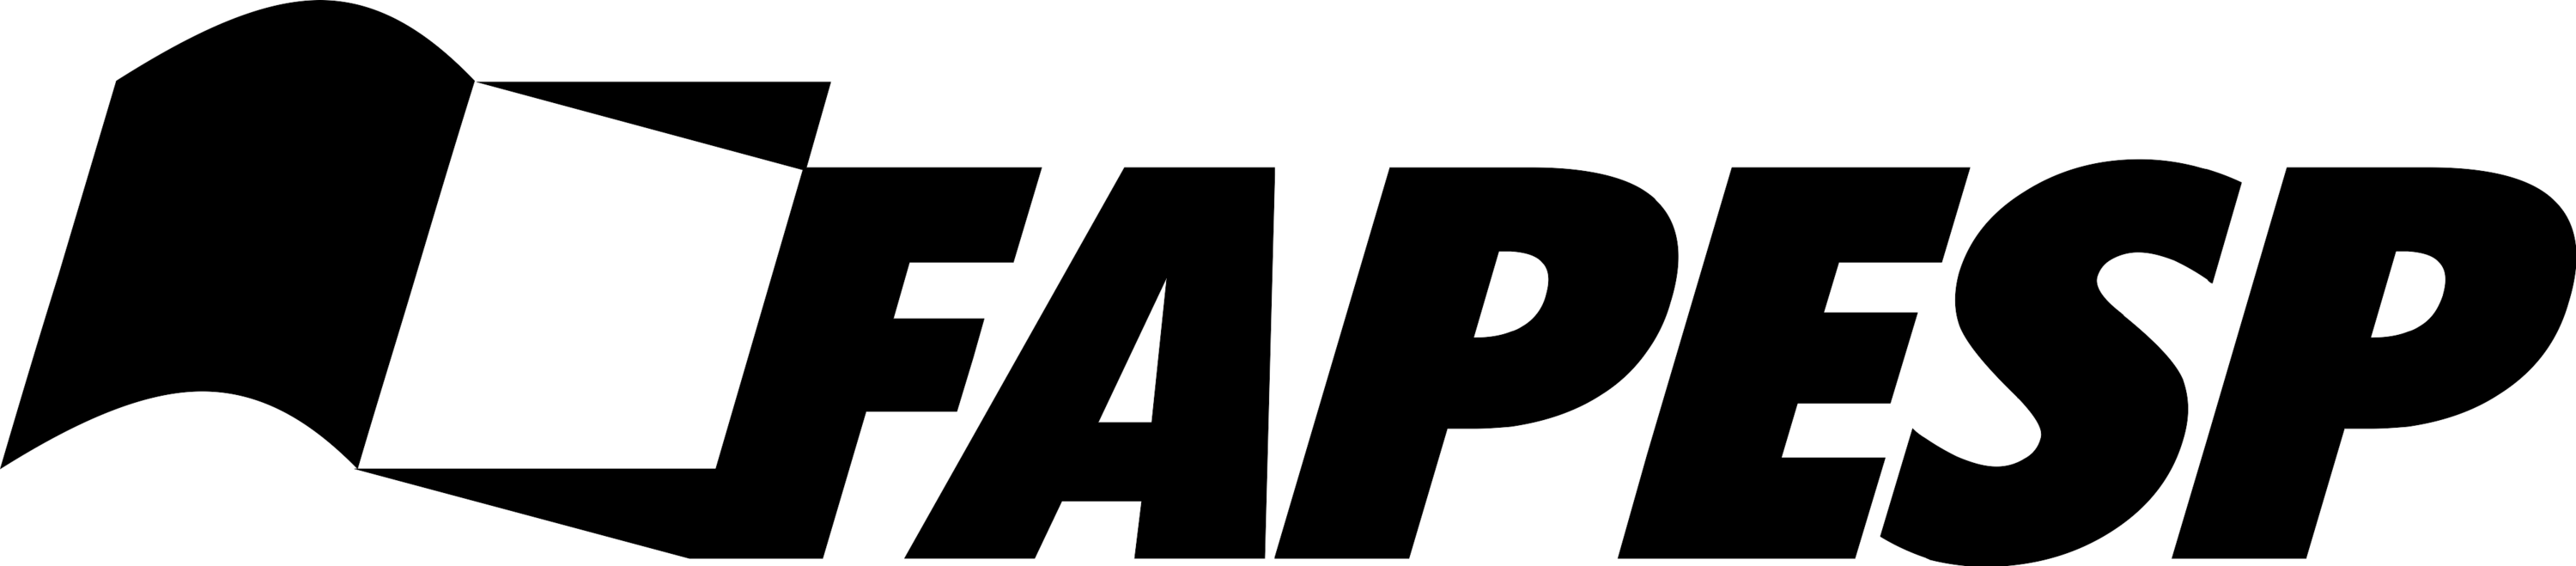
\includegraphics[width=\linewidth]{fapesp-logo.png}}
  \block{funding}{67.686}{15.144}{13.414}{\raggedleft\sffamily\fontsize{26}{31}\selectfont\color{Muted}Grant 2025/13861-1\par}
  \block{title}{3}{4.4}{55}{\sffamily\bfseries\fontsize{88}{96}\selectfont\color{Ink}Exact Algorithms for the\\Touring Polygons Problem}
  \block{subtitle}{3}{11.3}{55}{\sffamily\fontsize{34}{41}\selectfont\color{Muted}Shortest tours through polygonal regions, with proved bounds}
  \block{author}{3}{13.68}{37}{\sffamily\bfseries\fontsize{48}{55}\selectfont\color{Ink}Gabriel Freire Ushijima\par\vspace{0.08cm}\mdseries\fontsize{23}{27}\selectfont\color{Muted}\href{mailto:gabriel_ushijima@usp.br}{gabriel\_ushijima@usp.br} · IME-USP}
  \block{advisor}{30}{13.68}{37}{\sffamily\bfseries\fontsize{48}{55}\selectfont\color{Ink}Ernesto G. Birgin \mdseries(Advisor)\par\vspace{0.08cm}\fontsize{23}{27}\selectfont\color{Muted}\href{mailto:egbirgin@ime.usp.br}{egbirgin@ime.usp.br}}
  \draw[Rule,line width=1.1pt] (3,17.0) -- (81.1,17.0);

  % Row 1: the problem, and what was known and what we add.
  \draw[Rule,line width=0.8pt] (41.95,17.7) -- (41.95,36.9);
  \block{intro-head}{3}{17.7}{38.2}{\head{1}{Objectives}}
  \block{intro-context}{3}{19.50}{38.2}{\bodytext A drone must fly over each of Brazil's 27 federative units and return to where it started. In which \textbf{order}, and through which \textbf{point} of each region, is the route shortest? Touching or crossing a region counts as a visit. Area targets arise in delivery, surveillance and precision agriculture, and real regions are often non-convex.}
  \fill[Pale,rounded corners=0.22cm] (3,24.33) rectangle (20.4,28.49);
  \draw[Rule,line width=1.0pt,rounded corners=0.22cm] (3,24.33) rectangle (20.4,28.49);
  \block{tsp}{3.55}{24.83}{16.3}{{\sffamily\bfseries\fontsize{27}{32}\selectfont\color{Accent}TSP}\hspace{0.12cm}\raisebox{0.08cm}{{\sffamily\mdseries\fontsize{22}{26}\selectfont\color{Muted}·\hspace{0.12cm}Traveling Salesman Problem}}\par\vspace{0.10cm}\bodytext Shortest closed tour\\through a set of points.}
  \fill[Pale,rounded corners=0.22cm] (3,28.99) rectangle (20.4,34.05);
  \draw[Rule,line width=1.0pt,rounded corners=0.22cm] (3,28.99) rectangle (20.4,34.05);
  \block{tpp}{3.55}{29.49}{16.3}{{\sffamily\bfseries\fontsize{27}{32}\selectfont\color{Accent}TPP}\hspace{0.12cm}\raisebox{0.08cm}{{\sffamily\mdseries\fontsize{22}{26}\selectfont\color{Muted}·\hspace{0.12cm}Touring Polygons Problem}}\par\vspace{0.10cm}\bodytext Shortest path from $s$ that visits\\a sequence of polygons in order\\and ends at $t$.}
  \fill[Accent!7,rounded corners=0.24cm] (22.8,25.97) rectangle (41.1,32.41);
  \draw[Accent!65,line width=1.2pt,rounded corners=0.24cm] (22.8,25.97) rectangle (41.1,32.41);
  \block{free-order}{23.45}{26.47}{17.0}{{\tagtext TSPN · free-order tour}\par\vspace{0.14cm}\bodytext Shortest closed tour that visits\\a set of polygons in any order,\\with no fixed point.\par\vspace{0.10cm}\bodytext\bfseries This is the problem we solve.}
  \draw[Accent,line width=1.8pt,-{Stealth[length=3mm]}] (20.5,26.41) -- (22.7,28.7);
  \draw[Accent,line width=1.8pt,-{Stealth[length=3mm]}] (20.5,31.52) -- (22.7,29.7);
  \block{aim}{3}{34.75}{38.2}{\bodymuted\textbf{Aim:} an exact, self-contained solver for the TSPN, with no commercial optimizer, compared with the state of the art [3].}

  \block{background-head}{42.7}{17.7}{38.4}{\head{2}{Background and contribution}}
  \block{background}{42.7}{19.50}{38.4}{\tagtext A polynomial subproblem\par\vspace{0.15cm}\bodytext Both variants are NP-hard for non-convex polygons, but the fixed-order TPP with convex polygons is polynomial: Dror et al. [1] use last-step shortest-path maps, improved by Tan and Jiang [2]. These algorithms fix $s$ and $t$; a TSPN tour has no fixed point.\par\vspace{1.0cm}\tagtext The state of the art\par\vspace{0.15cm}\bodytext Fekete et al. [3] solve the TSPN by branch and bound. Each convex subproblem is a second-order cone program (SOCP) solved by Gurobi, a commercial optimizer, within a tolerance.\par\vspace{1.0cm}\tagtext Our contribution\par\vspace{0.15cm}\bodytext An exact algorithm for the \textbf{fixed-order closed tour} through convex polygons, which may touch or overlap, with \textbf{zero error on rational input}. We use it as the geometric oracle of an \textbf{exact branch-and-bound solver for the TSPN}, replacing the SOCP solver used in [3]. For speed, floating-point bounds are proved with directed rounding; the exact stage runs only when needed. On the 541 instances both solve with one thread, ours is faster on every instance, with a \textbf{69× median speedup} over the state of the art [3].}
  \draw[Rule,line width=1.1pt] (3,37.6) -- (81.1,37.6);

  % Row 2: the Brazil instance of the poster and the web page, and the search.
  \draw[Rule,line width=0.8pt] (37.75,38.3) -- (37.75,77.8);
  \block{map-head}{3}{38.3}{34}{\head{3}{Brazil as an instance}}
  \block{map-context}{3}{40.1}{34}{\bodytext 27 federative units with simplified borders. The shortest closed tour that crosses all: \textbf{9{,}962~km}, proved optimal in \textbf{0.02 s} with one thread; 10{,}039~km if forced through Brasília. Lighter: visited earlier, counting from the Federal District.}
  \block{map}{3}{43.8}{34}{\includegraphics[width=\linewidth]{brazil-route.pdf}}

  \block{method-head}{38.5}{38.3}{42.6}{\head{4}{Branch and bound}}
  \block{method}{38.5}{40.1}{42.6}{\bodytext A node holds a partial sequence of $m$ targets, each one its \textbf{convex hull} or one \textbf{convex piece} of an optimal decomposition by Greene's algorithm [4]. The node's closed tour is a \textbf{lower bound} $L$ for every extension, since omitting targets cannot lengthen a route; the best feasible length so far is $U$. The insertion and refinement rules follow [3].}
  \card{38.5}{44.9}{feasible}{method-01.pdf}{01 · Feasible tour}{\begin{tabular}{@{}l@{\hspace{0.5cm}}l@{}}Native heuristic & \tourkey{Accent}{solid}\\Final tour & \tourkey{Ink}{dash pattern=on 7pt off 4pt}\end{tabular}}
  \card{52.85}{44.9}{partial}{method-02.pdf}{02 · Partial order}{Dashed hulls fix A, B, C; D is visited incidentally.}
  \card{67.2}{44.9}{prune}{method-03.pdf}{03 · Prune}{If $L \ge U$, prune this branch.}
  \card{38.5}{61.6}{incumbent}{method-04.pdf}{04 · Update $U$}{Visits every region;\\a shorter tour lowers $U$.}
  \card{52.85}{61.6}{insert}{method-05.pdf}{05 · Insert}{$P$ goes into each of the $m$ gaps of the cycle.}
  \card{67.2}{61.6}{refine}{method-06.pdf}{06 · Refine}{Branch on B: one child per convex piece.}
  \draw[Rule,line width=1.1pt] (3,78.5) -- (81.1,78.5);

  % Row 3: results on the left, the web page on the right.
  \draw[Rule,line width=0.8pt] (59.5,79.2) -- (59.5,107.85);
  \block{results-head}{3}{79.2}{55.6}{\head{5}{Results on the 558 instances of Fekete et al.}}
  \block{results-context}{3}{81.0}{55.6}{\bodytext The original code of [3] and ours on one AMD Ryzen 7 9700X: three 300 s runs per setup, plus 900 s on open instances. Both stop at $U - L \le \varepsilon U + \varepsilon$, with $\varepsilon = 10^{-3}$ as in [3]; our bounds are proved.}
  \block{figure-2}{3}{83.65}{32}{\includegraphics[width=\linewidth]{speedup-figure.pdf}}
  \block{figure-2-caption}{3}{101.25}{32}{\bodymuted\textbf{Figure.} Speedup over [3], one thread each, on the 541 instances both solve; median and arithmetic mean by size, rounded to a multiple of 5.}
  \fill[white,rounded corners=0.30cm] (36.3,83.65) rectangle (58.6,88.85);
  \draw[Rule,line width=1.0pt,rounded corners=0.30cm] (36.3,83.65) rectangle (58.6,88.85);
  \draw[Route,line width=4.0pt] (36.6,83.70) -- (47.2,83.70);
  \draw[Accent,line width=4.0pt] (47.7,83.70) -- (58.3,83.70);
  \draw[Rule,line width=0.8pt] (47.45,84.10) -- (47.45,88.40);
  \block{median}{36.75}{84.30}{10.4}{\metric 69×\par\vspace{0.12cm}\bodytext\textbf{Median speedup}}
  \block{mean}{47.9}{84.30}{10.4}{\metric 183×\par\vspace{0.12cm}\bodytext\textbf{Arithmetic mean}}
  \block{gain}{36.3}{89.55}{22.3}{\tagtext Where the gain comes from\par\vspace{0.15cm}\bodytext On 166 cases both close in all three 300 s runs, where [3] takes $\ge$ 1 s (one thread each), fastest runs give \textbf{245×} speedup: [3] uses 1.08× as many nodes at \textbf{226×} the cost per node. Geometric means: $1.08 \times 226 \approx 245$.}
  \block{solved-table}{36.3}{95.45}{22.3}{\tagtext Instances solved\par\vspace{0.15cm}\sffamily\mdseries\fontsize{24}{29}\selectfont\color{Ink}\begin{tabular}{@{}p{12.4cm}@{\hspace{0.3cm}}r@{\hspace{0.5cm}}r@{}}\color{Muted}& \color{Muted}300 s & \color{Muted}900 s\\[0.1cm]{[3]}, 16 threads & 542 & 549\\{[3]}, one thread & 523 & 541\\\textbf{Ours, one thread} & \textbf{557} & \textbf{557}\end{tabular}\par\vspace{0.2cm}\bodymuted One instance remains open in 900 s for ours and every setup of [3].}
  \block{precision}{3}{103.9}{55.6}{\tagtext Accuracy\par\vspace{0.15cm}\bodytext One thread each; CHR for [3]. Largest polygon miss per instance over three 300 s runs: median $2.65\times10^{-6}$, max $8.23\times10^{-4}$ for [3], within its $10^{-3}$ tolerance. Ours stay within $3\times10^{-11}$; [3]'s upper bound lies below our proved lower bound on 22 instances.}

  \block{app-head}{60.4}{79.2}{20.7}{\head{6}{Try it yourself!}}
  \block{app-intro}{60.4}{81.0}{20.7}{\bodytext Scan to watch the tours, play the challenges and explore every result.}
  \fill[white,rounded corners=0.18cm] (60.4,83.65) rectangle (81.1,85.15);
  \draw[Rule,line width=0.8pt,rounded corners=0.18cm] (60.4,83.65) rectangle (81.1,85.15);
  \block{app-explore-title}{60.8}{84.10}{5.4}{\sffamily\bfseries\fontsize{26}{31}\selectfont\color{Accent}Watch}
  \block{app-explore-detail}{66.4}{84.10}{14.6}{\sffamily\fontsize{26}{31}\selectfont\color{Ink}Brazil · São Paulo · USP}
  \fill[Pale,rounded corners=0.18cm] (60.4,85.35) rectangle (81.1,86.85);
  \draw[Rule,line width=0.8pt,rounded corners=0.18cm] (60.4,85.35) rectangle (81.1,86.85);
  \block{app-challenge-title}{60.8}{85.80}{5.4}{\sffamily\bfseries\fontsize{26}{31}\selectfont\color{Accent}Play}
  \block{app-challenge-detail}{66.4}{85.80}{14.6}{\sffamily\fontsize{26}{31}\selectfont\color{Ink}3 interactive challenges}
  \fill[white,rounded corners=0.18cm] (60.4,87.05) rectangle (81.1,88.55);
  \draw[Rule,line width=0.8pt,rounded corners=0.18cm] (60.4,87.05) rectangle (81.1,88.55);
  \block{app-investigate-title}{60.8}{87.50}{5.4}{\sffamily\bfseries\fontsize{26}{31}\selectfont\color{Accent}Explore}
  \block{app-investigate-detail}{66.4}{87.50}{14.6}{\sffamily\fontsize{26}{31}\selectfont\color{Ink}All 558 instances of [3]}
  % Level-H correction leaves room for the TPP mark over the centre of the code.
  \block{qr}{62.15}{89.05}{17.2}{\qrcode[level=H,height=17.2cm]{\appurl}}
  \fill[white,rounded corners=0.2cm] (67.95,94.85) rectangle (73.55,100.45);
  \begin{scope}[shift={(68.25,95.15)},scale=0.078125]
    \fill[Ink,rounded corners=0.9375cm] (0,-0.55) rectangle (64,63.45);
    \draw[LogoTeal,line width=8.8pt,join=round] (32,9.45) -- (53,49.45) -- (11,49.45) -- cycle;
    \draw[Route,line width=7.7pt,line cap=round] (10,35.45) -- (54,28.45);
    \fill[white] (10,35.45) circle[radius=4];
    \fill[white] (54,28.45) circle[radius=4];
  \end{scope}
  \block{app-link}{60.4}{106.55}{20.7}{\centering\sffamily\bfseries\fontsize{20}{24}\selectfont\color{Accent}\href{\appurl}{yushipy.github.io/TouringPolygons/\\apps/siicusp34/en/}}

  % Conclusions span the full width above the references.
  \fill[Pale,rounded corners=0.20cm] (3,108.45) rectangle (81.1,112.30);
  \draw[Rule,line width=0.8pt,rounded corners=0.20cm] (3,108.45) rectangle (81.1,112.30);
  \draw[Accent,line width=3.0pt] (3.3,108.50) -- (80.8,108.50);
  \block{conclusion}{3.7}{108.95}{76.7}{\bodytext\textbf{\color{Accent}Conclusions.} An exact algorithm for the fixed-order closed tour through convex polygons, with zero error on rational input, is the core of an exact branch-and-bound solver for the TSPN. It is one to two orders of magnitude faster than the state of the art and closes 557 of 558 benchmark instances with proved bounds, without a commercial optimizer. Next: disk neighborhoods (Close-Enough TSP) and vehicle routing with polygonal neighborhoods.}

  % References; the digital PDF keeps live links.
  \block{references-col-1}{3}{112.90}{25.3}{\sffamily\fontsize{20}{24}\selectfont\color{Muted}[1] Dror, Efrat, Lubiw, Mitchell. \href{https://doi.org/10.1145/780542.780612}{\emph{Touring a sequence of polygons}}. STOC, 2003.\par [2] Tan, Jiang. \href{https://doi.org/10.1007/978-3-319-55911-7_44}{\emph{Efficient algorithms for touring a sequence of convex polygons}}. TAMC, 2017.}
  \block{references-col-2}{29.4}{112.90}{25.3}{\sffamily\fontsize{20}{24}\selectfont\color{Muted}[3] Fekete, Kniep, Krupke, Perk. \href{https://doi.org/10.4230/LIPIcs.SoCG.2026.46}{\emph{A branch-and-bound algorithm for the Traveling Salesman Problem with difficult neighborhoods}}. SoCG, 2026.}
  \block{references-col-3}{55.8}{112.90}{25.3}{\sffamily\fontsize{20}{24}\selectfont\color{Muted}[4] Greene. \emph{The decomposition of polygons into convex parts}. Computational Geometry, JAI Press, 1983.\par\textbf{The author declares no conflict of interest.}}
\end{tikzpicture}
\end{document}
